\documentclass[border=5mm]{standalone}
\usepackage[utf8]{inputenc}
\usepackage[T1]{fontenc}
\usepackage{amsmath}
\usepackage{tikz}
\usepackage{pgfplots}
\pgfplotsset{compat=1.18}
\usetikzlibrary{arrows.meta}
\definecolor{utnblue}{RGB}{0, 51, 102}

% Ej8 signals: x(t) = u(t)·u(1-t)        (pulso rectangular en [0,1])
%              h(t) = t·u(t)·u(2-t)      (rampa lineal truncada en [0,2])
% Mismo tamaño de panel y mismas escalas que fig_ej8_zonas.

\begin{document}
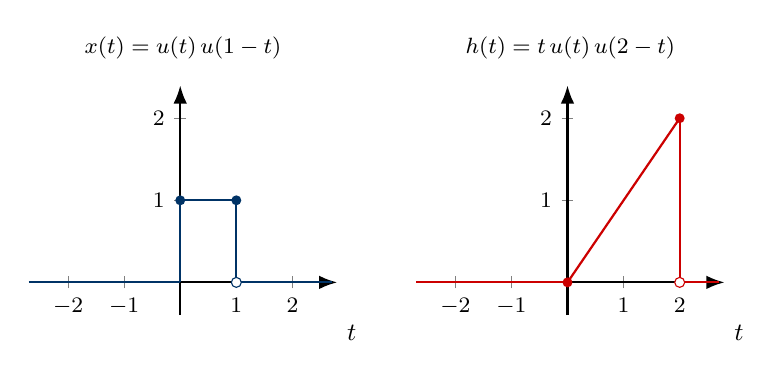
\begin{tikzpicture}[>=Latex, font=\small]

\colorlet{xcol}{utnblue}
\colorlet{hcol}{red!80!black}

\pgfmathsetmacro{\tmin}{-2.7}
\pgfmathsetmacro{\tmax}{2.8}

% =====================================================================
% PANEL x(t)
% =====================================================================
\begin{axis}[
    name=panX,
    width=5.5cm, height=4.5cm,
    axis lines=center,
    xlabel={$t$},
    xlabel style={anchor=north west, at={(axis description cs:1,0)}},
    xmin=\tmin, xmax=\tmax,
    ymin=-0.4, ymax=2.4,
    clip=false,
    axis line style={->, thick},
    xtick={-2,-1,0,1,2},
    ytick={0,1,2},
    every tick label/.style={font=\footnotesize},
    title={\footnotesize $x(t) = u(t)\,u(1-t)$},
]
    % cero a la izquierda
    \addplot[xcol, thick, domain=\tmin:0, samples=2] {0};
    % pulso = 1 en [0,1]
    \addplot[xcol, thick, domain=0:1, samples=2] {1};
    % cero a la derecha de 1
    \addplot[xcol, thick, domain=1:{\tmax-0.1}, samples=2] {0};
    % salto en t=0: 0 -> 1
    \draw[xcol, thick] (axis cs:0,0) -- (axis cs:0,1);
    \fill[xcol] (axis cs:0,1) circle (1.8pt);
    % salto en t=1: 1 -> 0 (u(0)=1: relleno arriba, abierto abajo)
    \draw[xcol, thick] (axis cs:1,0) -- (axis cs:1,1);
    \fill[xcol]  (axis cs:1,1) circle (1.8pt);
    \fill[white] (axis cs:1,0) circle (1.8pt);
    \draw[xcol]  (axis cs:1,0) circle (1.8pt);
\end{axis}

% =====================================================================
% PANEL h(t)
% =====================================================================
\begin{axis}[
    name=panH,
    at={(panX.east)}, anchor=west, xshift=1cm,
    width=5.5cm, height=4.5cm,
    axis lines=center,
    xlabel={$t$},
    xlabel style={anchor=north west, at={(axis description cs:1,0)}},
    xmin=\tmin, xmax=\tmax,
    ymin=-0.4, ymax=2.4,
    clip=false,
    axis line style={->, thick},
    xtick={-2,-1,0,1,2},
    ytick={0,1,2},
    every tick label/.style={font=\footnotesize},
    title={\footnotesize $h(t) = t\,u(t)\,u(2-t)$},
]
    % cero a la izquierda
    \addplot[hcol, thick, domain=\tmin:0, samples=2] {0};
    % rampa en [0,2]
    \addplot[hcol, thick, domain=0:2, samples=2] {x};
    % cero a la derecha de 2
    \addplot[hcol, thick, domain=2:{\tmax-0.1}, samples=2] {0};
    % salto en t=2: h(2)=2 -> 0
    \draw[hcol, thick] (axis cs:2,0) -- (axis cs:2,2);
    \fill[hcol]  (axis cs:2,2) circle (1.8pt);
    \fill[white] (axis cs:2,0) circle (1.8pt);
    \draw[hcol]  (axis cs:2,0) circle (1.8pt);
    % continuidad en t=0
    \fill[hcol] (axis cs:0,0) circle (1.8pt);
\end{axis}

\end{tikzpicture}
\end{document}
